\documentclass{report}
\usepackage[utf8]{inputenc}
\usepackage[czech]{babel}
\usepackage{graphicx, import}
\usepackage{float}

\usepackage{color}

%tabulka%
\usepackage[table]{xcolor}
\usepackage{tabu}

% matematicke rovnice %
\usepackage{amsmath}

%hezke cisla v textu%
\usepackage{siunitx}

%odkazy%
\usepackage{hyperref}
%svg%
\usepackage{svg}



%vicesloupcova sazba%
\usepackage{multicol}
\usepackage{sidecap}
%citace%
\bibliographystyle{IEEEtran} 


\title{Deskriptor}
\author{Kateřina Kratochvílová}
% #########
% # START #
% #########

\begin{document} 
\shorthandoff{-}
% titulní stránka
%\maketitle
\begin{titlepage}
	\begin{flushleft} 
		{
\includegraphics[width=.5\textwidth]{./img/fav_logo.jpg}\\[3cm]}
	\end{flushleft}
	\vspace{1.5cm}
	\begin{center}
		{\Huge KIV/UIR - Semestrální práce}
	\end{center}
	\vfill
	{\normalsize 
		\today \hfill Kateřina Kratochvílová \\
		40 hodin \hfill A13B0364P \\
	}

\end{titlepage}


% obsah
\tableofcontents
\thispagestyle{empty} %odstraneni cisla stranky z obsahu

% abstrakt
\begin{abstract}
Tato práce byla vytvořena za účelem vytvoření deskriptoru, který ponese informaci nejeno o barvě, ale i o textuře obrázku. 
\end{abstract}

\chapter{Úvod}
Většina metod používaných na detekci textury pracuje pouze s šedotónovým obrázkem. Takže zanedbávají informaci o barvě a pracují jen s intenzitou obrazu. Cílem této práce však je obě informace zkombinovat a vytvořit tak jeden deskriptor, který ponese jak informaci o barvě tak i informaci o textuře obrázku \cite{DiplomovaBrno}. Nabízí se několik možností: 

\begin{description}
\item[Vytvoření společného příznaku] 
například rozšíření LBP/POEM na všechny barvené kanály. Musí se však dbát na to, že informace o barvě a textuře se mohou ovlinovat i protichůdně. 

\item[Vyhodnotit a klasifikovat příznaky odděleně] 
a pak výslednou klasifikaci spojit z několika částí (například JEC - Joint Equal Contribution \cite{JEC} ). Výhodou tohoto přístupu je zachování vlastností obou původních příznaků. Nevýhodou je náročnější výpočet a úspěšnost přístupu závisí na způsobu kombinace obou informací.
\end{description} 

V práci je rozebrán POEM (Patterns of Oriented Edge Magnitudes) pracující jen s texturou následovaný metodou POEM procházející všechny kanály barevného prostoru RGB. \\

Hotový deskriptor bude použit pro porovnání v bakalářské práci "Automatická anotace obrázků". Kde hlavním tématem je právě spojení příznaků vyhodnocených zvlášť. 

\chapter{Poem}
POEM (Patterns of Oriented Edge Magnitudes). Vstup algorimutmu se předpokládá šedotónový obrázek o rozměrech  $m \times n$. Proto každý obrázek musí být po načtení převeden na šedotóny, protože většinou vkládáme obrázek barevný. \cite{SrovnaniDeskriptoru}

\subsection{Výpočet gradientu a magnitudy}
Nejprve je potřeba vypočítat gradient. Gradient je obecně směr růstu. Výpočet může probíhat různými způsoby. Jednou z možností je použít masku, kterou aplikujeme na vstupní obrázek. Podle některých studii jsou nejlepší jednoduché masky jako je např. $[1, 0, -1]$ a $[1, 0, -1]^{\,t}$. Okraje obrázku se buď vypouštějí nebo se dají doplnit (opět existuje více způsobů).Výstupem jsou dva obrázky o rozměrech $m \times n$. \\
Na výstup se dá pohlížet také jako na vektory, kdy každý bod původního obrázku je reprezentován právě 2D vektorem. Analogicky pokud si vektory rozložíme na x a y složku dostaneme dva obrázky. Jeden, který reprezentuje obrázek po použití x-ového filtru, a druhý který reprezentuje obrázek po použití y-filtru. Přičemž použití y filtru by nám mělo zvýraznit hrany v y směru (svislé) a x zvýrazní hrany v x směru (vodorovné). \\

\begin{multicols}{2}
	Vstupní obrázek:
 	\begin{center}
  		\begin{tabular}{ | l | c | r | }
    		\hline
    		8 & 7 & 5 \\ \hline
    		1 & 2 & 4 \\ \hline
    		3 & 5 & 7 \\
    		\hline
  		\end{tabular}
  	\end{center}
  	Masky: 
	\begin{align*}
  		maska(x) &= 
  		\begin{tabular}{ | c | c |  }
    		\hline
    		-1 & 1 \\
    		\hline
  		\end{tabular}
  		\\
  		maska(y) &=
  		\begin{tabular}{ | c |  }
    		\hline
    		-1 \\ \hline
     		1 \\
    		\hline
  		\end{tabular}   
	\end{align*}
\end{multicols}
\vspace{3cm}
Na základě předchozích masek a vstupního obrázku byly vypočteny tyto matice gradientů:
\begin{multicols}{2}
	Pro x:
 	\begin{center}
  		\begin{tabular}{ | c | c | c | }
    		\hline
    		-1 & -2 & 0 \\ \hline
    		1 & 2 & 0 \\ \hline
    		2 & 2 & 0 \\
    		\hline
  		\end{tabular}
  	\end{center}
  	Pro y:
  	\begin{center}
  		\begin{tabular}{ | c | c | c | }
    		\hline
    		-7 & -5 & -1 \\ \hline
    		2 & 3 & 3 \\ \hline
    		0 & 0 & 0 \\
    		\hline
  		\end{tabular}
  	\end{center} 	
\end{multicols}

Gradient jako 2D vektory:
\begin{center}
  \begin{tabular}{ | c | c | c | }
    \hline
    [-1 ; -7] & [-2 ; -5] & [0 ; -1] \\ \hline
    [1 ; 2] & [2 ; 3] & [0 ; 3] \\ \hline
    [2 ; 0] & [2 ; 0] & [0 ; 0] \\
    \hline
  \end{tabular}
\end{center}

Magnituda je velikost směru růstu, lze si ji představit jako velikost směru růstu pro každý pixel (počítá se tedy pro každý pixel).  Z toho vyplývá, že ji můžeme spočítat jako velikost 2D vektorů, které jsme dostaly při výpočtu gradientu. Zjednodušeně magnituda představuje velikost vektoru gradientu. \\

Vzoreček pro výpočet velikosti vektoru v rovině:
\begin{align}
   \label{velikost_vektoru} |u| = \sqrt{u_1^2 + u_2^2}
\end{align}

Magnituda na základě vyše uvedených gradientů:
\begin{center}
  \begin{tabular}{ | c | c | c | }
    \hline
    7.1 & 5.4 & 1.0 \\ \hline
    2.2 & 3.6 & 3.0 \\ \hline
    2.0 & 2.0 & 0.0 \\
    \hline
  \end{tabular}
\end{center}

\begin{figure}[H]
	\centering
	\begin{minipage}[c]{150pt}
		\centering
		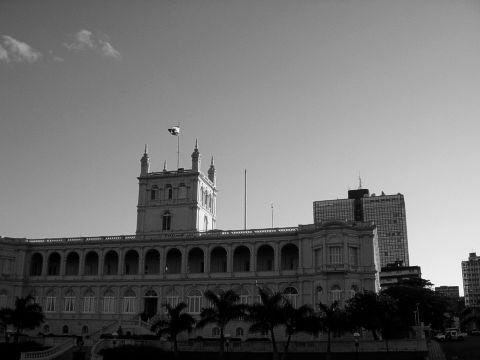
\includegraphics[width=150pt]{./img/vstupni_obraz.jpg}
		\caption{Vstupní obrázek}
	\end{minipage}
	\begin{minipage}[c]{150pt}
		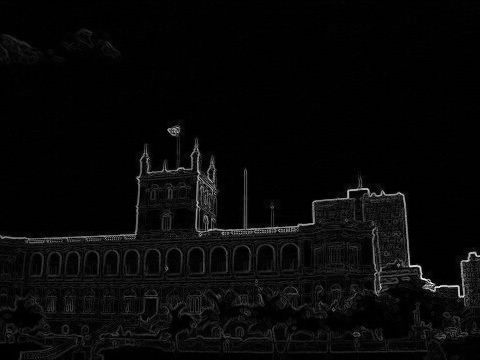
\includegraphics[width=150pt]{./img/magnitude.jpg}
		\caption{magnituda}
		\centering
	\end{minipage}
\end{figure}

\begin{figure}[H]
	\centering
	\begin{minipage}[c]{150pt}
		\centering
		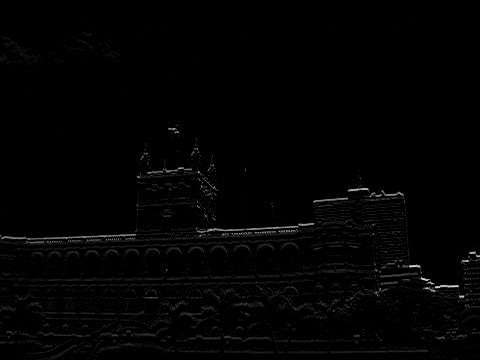
\includegraphics[width=150pt]{./img/gradientX.png}
		\caption{gradient x}
	\end{minipage}
	\begin{minipage}[c]{150pt}
		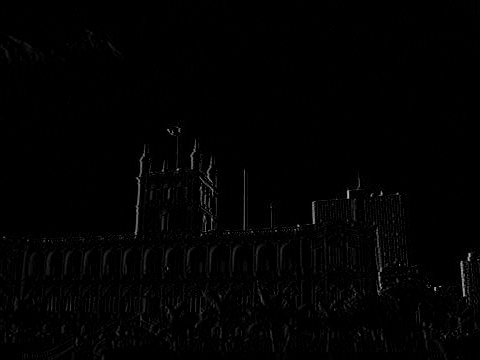
\includegraphics[width=150pt]{./img/gradientY.png}
		\caption{gradient y}
		\centering
	\end{minipage}
\end{figure}

\subsection{Diskretizace směru gradientu}
Pokud se na gradienty bude pohlížet jako na 2D vektory a tím určit nejen jejich velikost(magnitudu) ale i jejich směr. Je možné použít znaménkovou reprezentaci $0 - \pi$ nebo neznaménkovou reprezentaci $0 - 2\pi$. \\
V praxi si rovnoměrně rozdělíme kružnici na několik dílů (dle počtu požadovaných směrů). Počet dílů  je označen písmenem $d$. Pro $d = 3$ znaménkovou reprezentaci to tedy bude $\left(0 - \frac{2}{3}\pi \right)$, $\left(\frac{2}{3}\pi - \frac{4}{3}\pi \right)$ a $\left(\frac{4}{3}\pi - 2\pi \right)$. Je připraveno $d$ matic (pro každý směr jedna) a podle toho kam vektor směřuje, umístíme jeho magnitudu na souřadnice kde se nachází v původní matici. 

\begin{figure}[H]
    \centering    
    \def\svgwidth{230pt}
	\import{img/}{2D_kruznice.pdf_tex}    
    %\input{image.pdf_tex}
    \caption{Diskretizace směru gradientu. Každá barva představuje jeden směr šedá: $\left(0 - \frac{2}{3}\pi \right)$ , zelená:$\left(\frac{2}{3}\pi - \frac{4}{3}\pi \right)$ a žlutá: $\left(\frac{4}{3}\pi - 2\pi \right)$. Vektor $[ -2, -5 ]$ směřuje do třetího směru, proto uložíme jeho magnitudu do třetí matice. }
    \label{fig: 2D_graf}
\end{figure}

\begin{figure}[H]
	\centering
	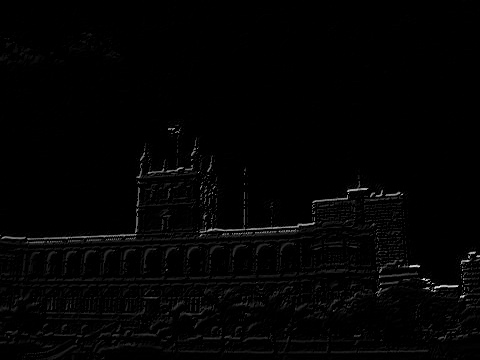
\includegraphics[width=150pt]{./img/directional0.jpg}
	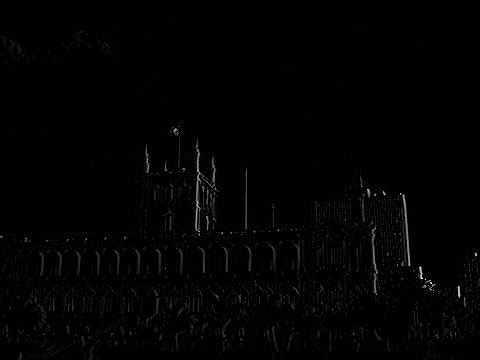
\includegraphics[width=150pt]{./img/directional1.jpg}
	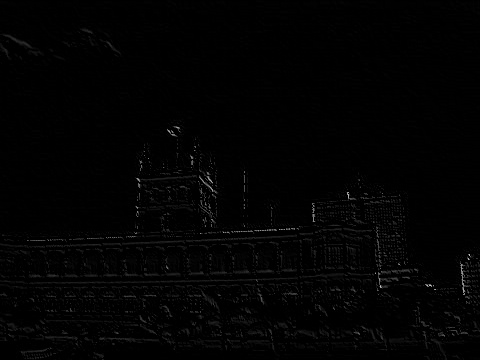
\includegraphics[width=150pt]{./img/directional2.jpg}
	\caption{Obrázky po diskretizaci. Každý obrázek představuje jeden směr.}
\end{figure}


\subsection{Výpočet lokálního histogramu orientace gradientů z okolí}
U každého směru  se vemou jednotlivé pixely s jejich okolím a zprůměrují se jejich hodnoty. Toto okolí se nazývá cell. \\

\definecolor{orange}{rgb}{1,0.5,0} 
Výpočet u jednoho směru při cell = 3, Oranžově je vyznačená oblast výpočtu pro jeden pixel:
\begin{multicols}{2}
	Vybraný směr:
 	\begin{center}
  		\begin{tabular}{ | c | c | c | c | }
    		\hline
    		0 & 0 & 0 & 0 \\ \hline
    		\cellcolor{orange!50}0 & \cellcolor{orange!50}0 & \cellcolor{orange!50}0 & 0 \\ \hline
    		\cellcolor{orange!50}0 & \cellcolor{orange!50}0 & \cellcolor{orange!50}0 & 0 \\ \hline
    		\cellcolor{orange!50}0 & \cellcolor{orange!50}3.6 & \cellcolor{orange!50}3.6 & 3 \\ \hline
    		0 & 2 & 2 & 0 \\
    		\hline
  		\end{tabular}
  	\end{center}
  	Jeho aems: 
  	\begin{center}
  		\begin{tabular}{ | c | c | }
    		\hline
    		0 & 0 \\ \hline
    		\cellcolor{orange!50}0.8 & 1.1 \\ \hline
    		1.2 & 1.5 \\
    		\hline
  		\end{tabular}
  	\end{center} 	
\end{multicols}

\begin{figure}[H]
	\centering
	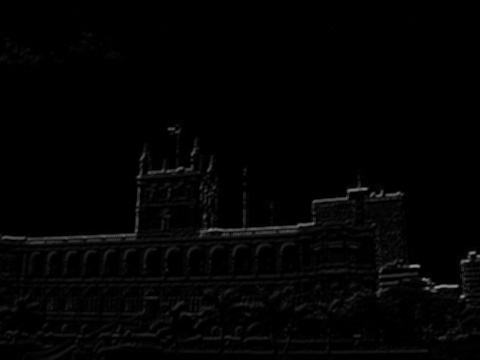
\includegraphics[width=150pt]{./img/aems0.jpg}
	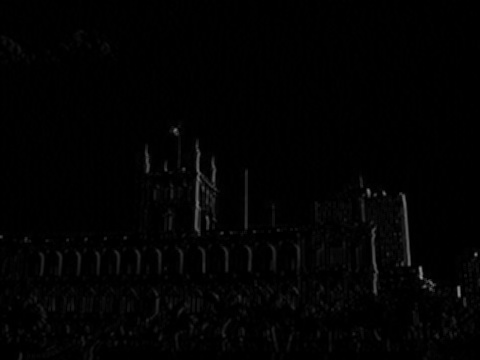
\includegraphics[width=150pt]{./img/aems1.jpg}
	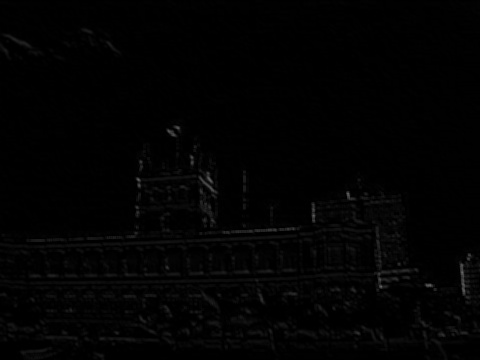
\includegraphics[width=150pt]{./img/aems2.jpg}
	\caption{Obrázky po diskretizaci, oproti předchozím jsou hrany více rozmazané. Každý obrázek představuje jeden směr.}
\end{figure}

\subsection{Zakódování příznaků pomocí LBP}
LBP operátor je aplikován na okolí každého pixelu o velikost $3 \times 3$. Oproti tomu POEM je možné aplikovat na větší okolí. Toto okolí se nazývá block, zpravidla se jedná o kruhové okolí s poloměrem L/2 (L představuje velikost blocku). Pro stanovení intenzit okolních hodnot je možné použít bilineární interpolaci. Pro zvýšení stability v téměř konstantní oblasti lze k centrálnímu pixelu přičítat malou konstantu $\tau$. 

\begin{figure}[H]
		\centering
		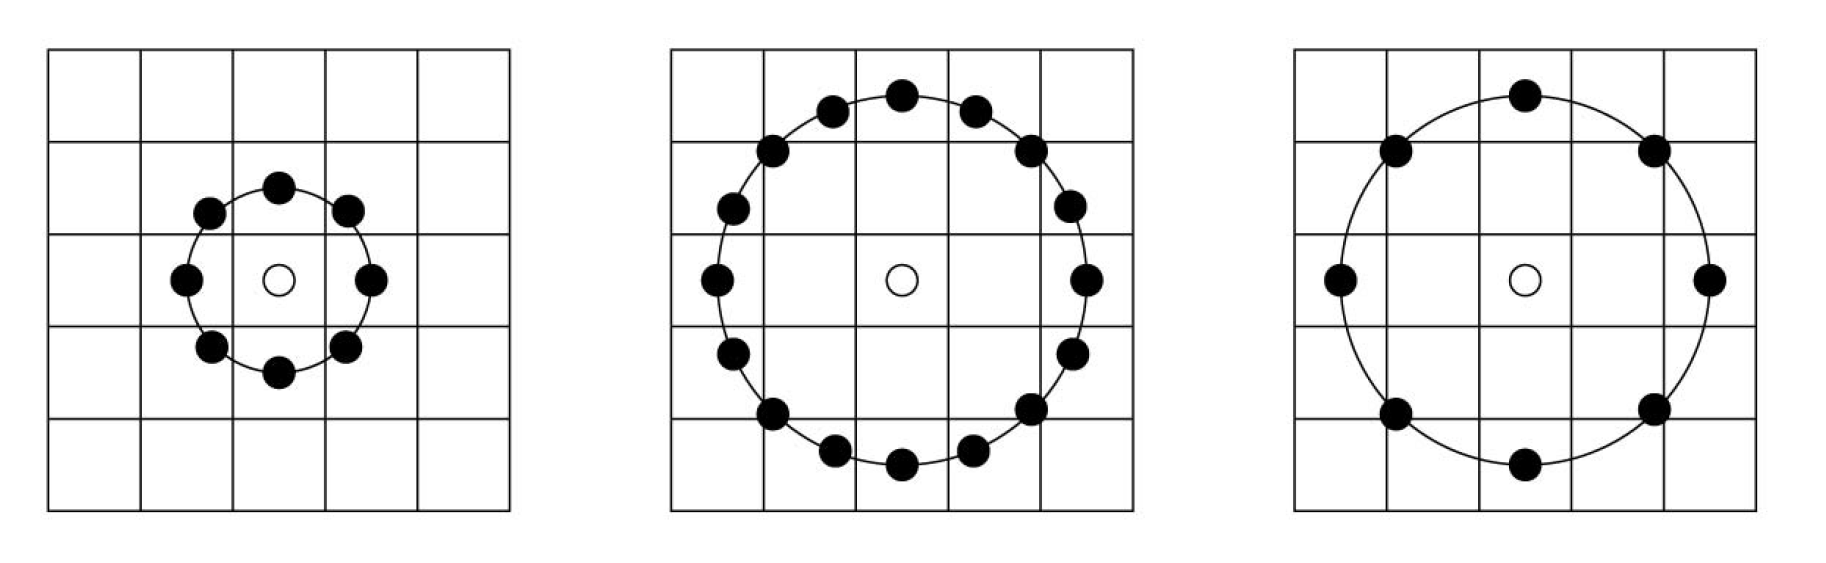
\includegraphics[width=253px]{./img/znazorneni_lbp.png}	
		\caption{Znázornění blocku Převzato z \cite{SrovnaniDeskriptoru}}
\end{figure}

Následující matice představuje block pro střední pixel s hodnotou intenzity 4, označený písmenem $c$ (centrální). Algoritmus následně prochází všechny okolní pixely, označené písmenem  $x$, hodnotu daného pixelu jako $p(x)$. $s(x)$ představuje výsledek tohoto porovnání.

\begin{displaymath} 
	\label{asd2} 
		    s(x) = \left\{ \begin{array}{r@{\quad}c}
    		1, & p(x) \geq h(c) \\
    		0, & p(x) < h(c) \\ \end{array} \right. 
\end{displaymath}

Zobrazení postupu algoritmu LBP: 
\begin{figure}[H]
		\centering
		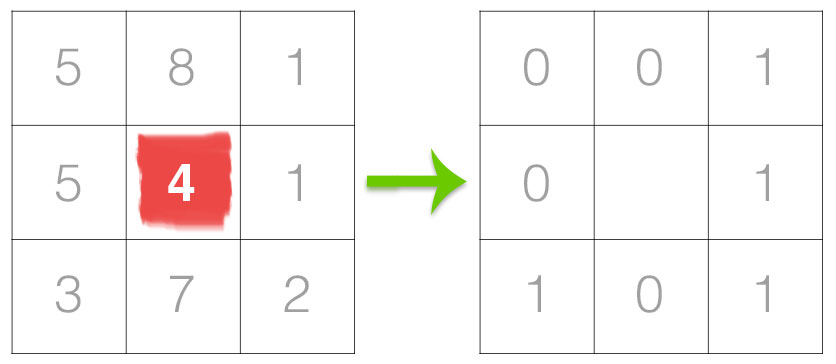
\includegraphics[width=200px]{./img/lbp_thresholding.jpg}
		\\[0.5cm]	
		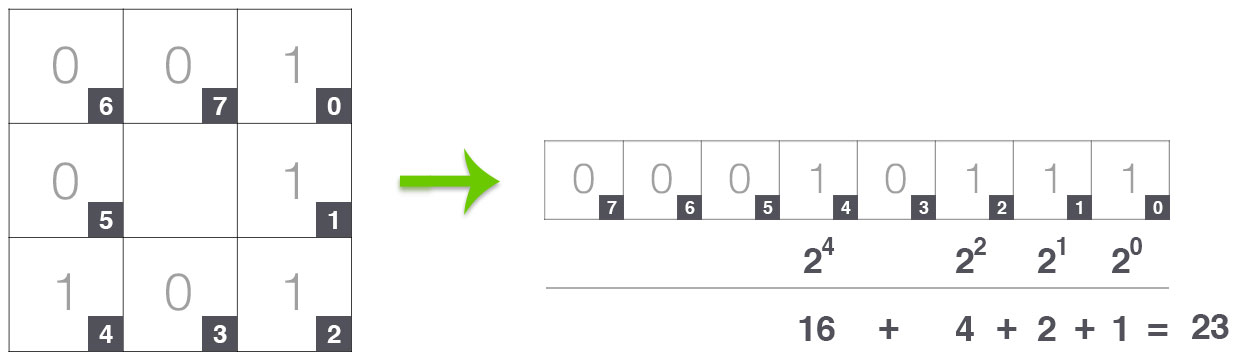
\includegraphics[width=350px]{./img/lbp_calculation.jpg}
		\\[0.5cm]
		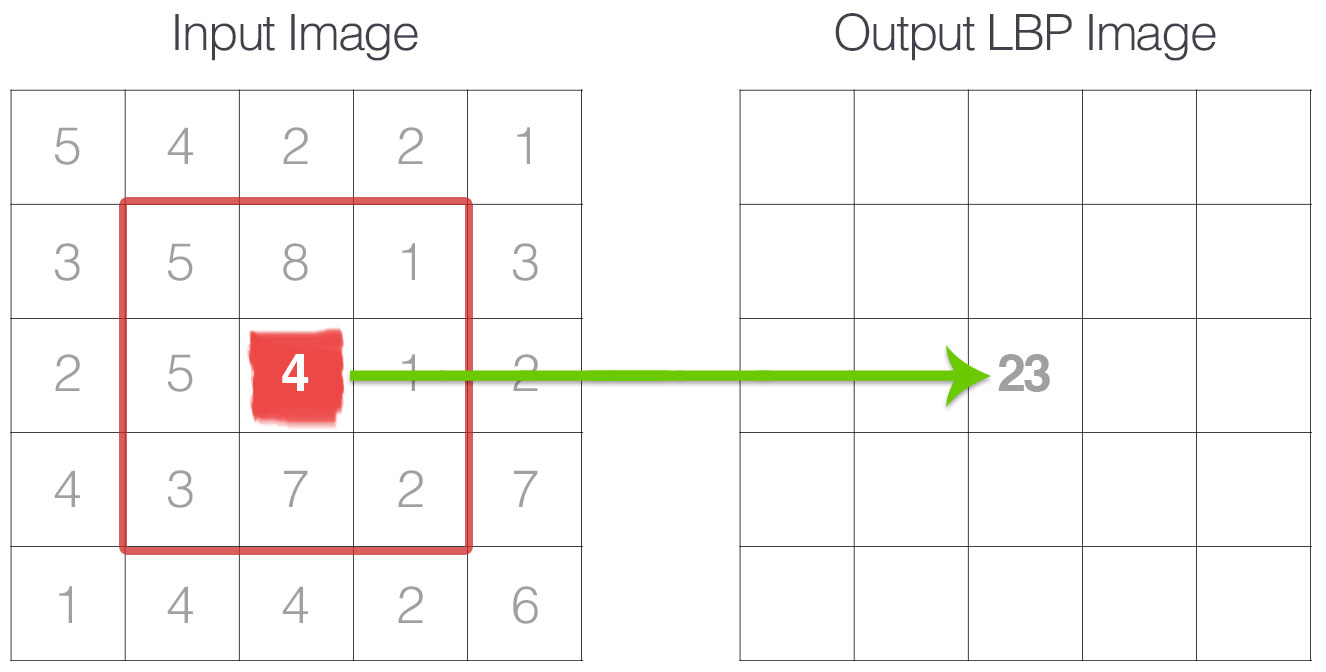
\includegraphics[width=253px]{./img/lbp_to_output.jpg}	
		\caption{Znázornění výpočtu LBP pro jeden pixel. Převzato z \cite{Pyimagesearch}}
\end{figure} 
 
\begin{figure}[H]
	\centering
	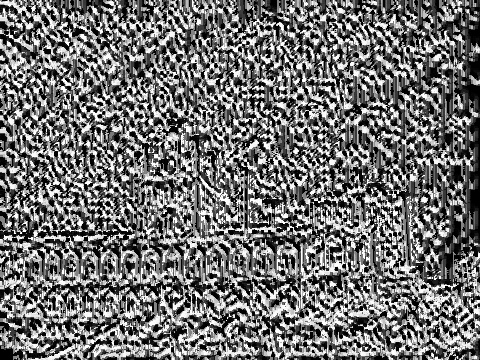
\includegraphics[width=150pt]{./img/lbp1.jpg}
	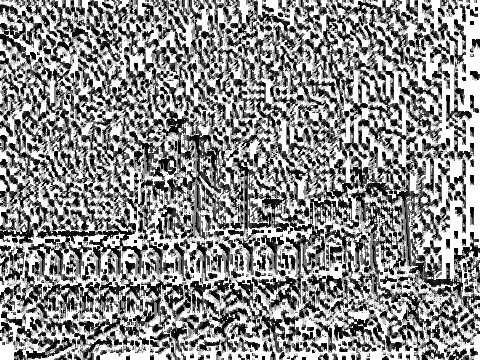
\includegraphics[width=150pt]{./img/lbp2.jpg}
	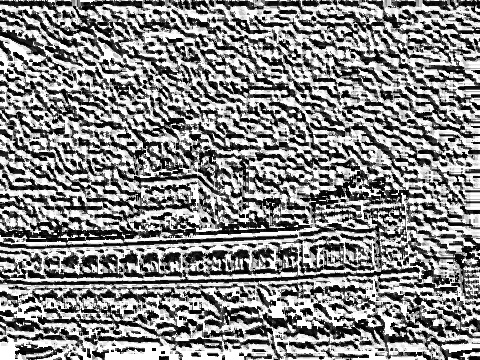
\includegraphics[width=150pt]{./img/lbp3.jpg}
	\caption{Obrázky po aplikaci LBP s velikostí blocku 8. Každý obrázek představuje jeden směr.}
\end{figure}

\begin{figure}[H]
	\centering
	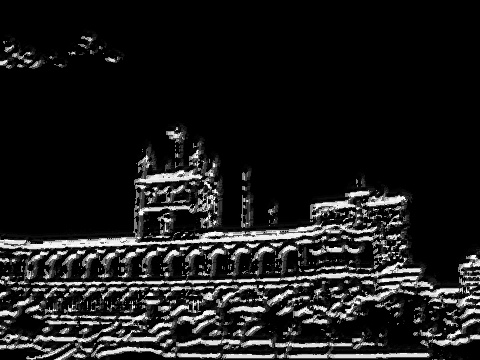
\includegraphics[width=150pt]{./img/lbp0_tau.jpg}
	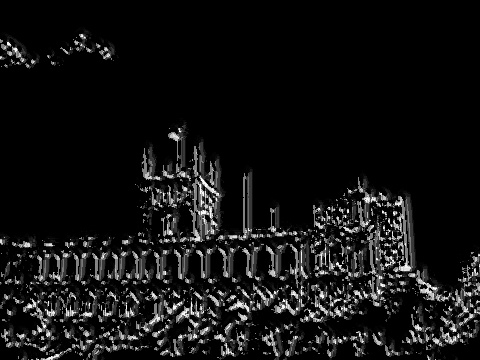
\includegraphics[width=150pt]{./img/lbp1_tau.jpg}
	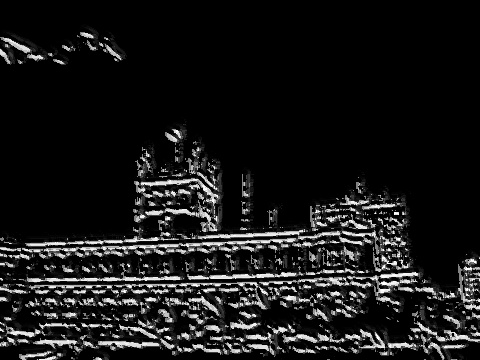
\includegraphics[width=150pt]{./img/lbp2_tau.jpg}
	\caption{Obrázky po aplikaci LBP při použití $\tau$. Každý obrázek představuje jeden směr.}
\end{figure} 

\subsection{Konstrukce globálního histogramu}
Obrázky získané z LBP jsou rozdeleny pravidelnou čtvercovou mřížkou. Pro každou vzniklou oblast je vypočten lokální histogram. Vzniklé histogramy jsou zřetězeny. Díky tomu jsou získány tři histogramy pro každý směr jeden, které jsou opět zřetězeny. \\
Rozdělení obrázků a určování lokálních histogramů se dělá za účelem zachování informace o prostorovém rozložení jednotlivých příznaků.

\subsubsection{Uniformní vzory}
Jelikož histogram, který bude vytvořen je velmi dlouhý, je možné ho zkrátit vybíráním pouze tz. uniformních vzorů. Některé binární vzory se totiž na běžných obrázcích vyskytují častěji a to až, dle experimentů z 90 \%. Jsou to právě výše zmíněné uniformní vzory. Uniformní vzory jsou hodnoty čísla (čísla z pohledu binární reprezentace), kdy dochází k maximálně dvěma přechodům z 0 na 1 a nebo opačně. Například 00011110 je uniformní, oproti tomu 01101111 není. Těchto vzorů je 58, všechny ostatní vzory jsou reprezentovány jediným vzorem. Takto je délka jednoho lokálního histogramu zredukována z 256 na 59 binů.

\begin{figure}[H]
	\centering
	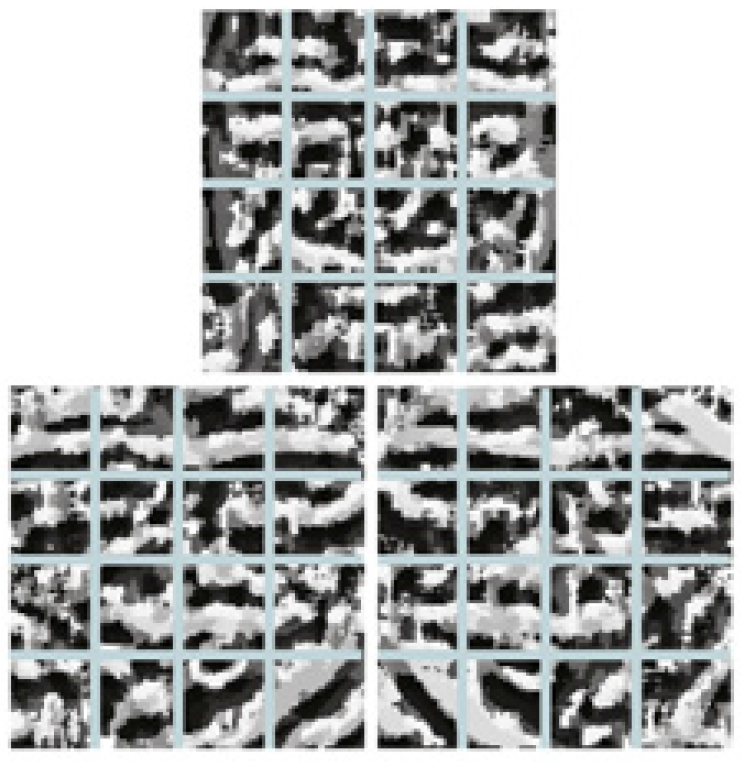
\includegraphics[width=150pt]{./img/vypocet_histogramu.png}
	\caption{Obrázky získané z LBP jsou rozděleny pravidelnou čtvercovou mřížkou. Převzato z \cite{SrovnaniDeskriptoru}}
\end{figure} 
\chapter{Barevný poem}

\subsection{Výpočet gradientu a magnitudy u barevneho poemu}
Výpočet gradientu probíhá obdobně jako u nebarevného obrázku. Pro každou ze tří složek jsou získány dvě matice filtrované maskami. Celkem bude $3 \times 2$ matic. Na matice se dá pohlížet jako na 2 vektory o 3 složkách. Vektory jsou sloučeny pomocí součtu vektoru do jednoho 3 složkového vektoru. Magnituda je opět velikost vektoru tentokrát, ale v prostoru. \\

Format vzniklych vektoru
\begin{align} 
	\label{bgr_vektory} 
		    u = [ blue_x, green_x, red_x ] \\ 
		    v = [ blue_y, green_y, red_y ] 
\end{align}

\begin{figure}[H]
		\centering
		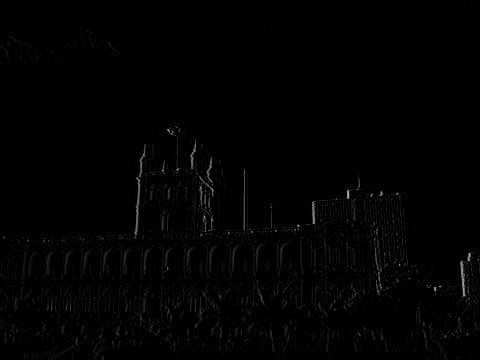
\includegraphics[width=150px]{./img/gradient_b_x.jpg}	
		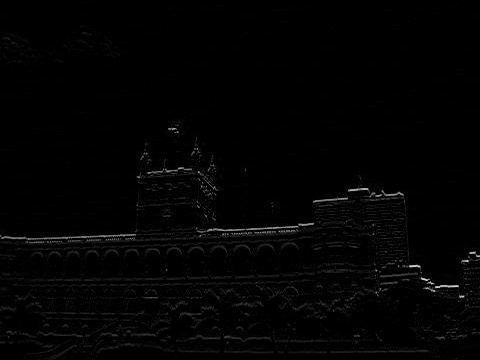
\includegraphics[width=150px]{./img/gradient_b_y.jpg}	
		\caption{Gradienty pro modrou složku.}
\end{figure}
\begin{figure}[H]
		\centering
		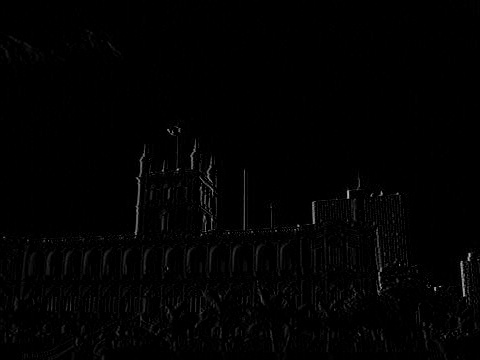
\includegraphics[width=150px]{./img/gradient_g_x.jpg}	
		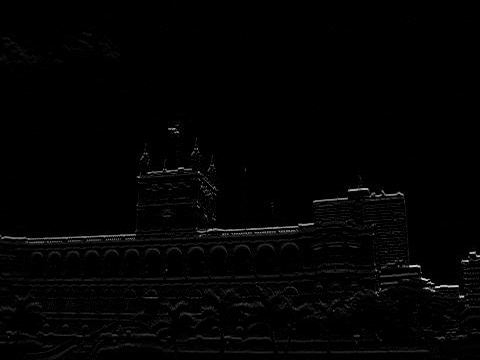
\includegraphics[width=150px]{./img/gradient_g_y.jpg}	
		\caption{Gradienty pro červenou složku}
\end{figure}
\begin{figure}[H]
		\centering
		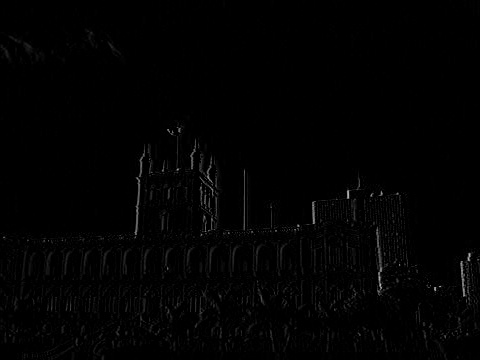
\includegraphics[width=150px]{./img/gradient_r_x.jpg}	
		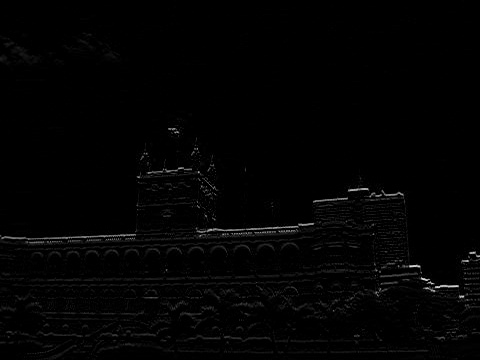
\includegraphics[width=150px]{./img/gradient_r_y.jpg}	
		\caption{Gradienty pro zelenou složku.}
\end{figure}

Pomocí součtu vektorů je získán jeden třísložkový vektor:
\begin{align}
   \label{soucet_vektrou} \vec{u} + \vec{v} = (u_1 + v_1, u_2 + v_2, u_3 + v_3 )
\end{align} 

Výpočet velikosti vektoru v prostoru (magnituda):
\begin{align}
   \label{velikost_vektoru_v_prostoru} |u| = \sqrt{u_1^2 + u_2^2 + u_3^2}
\end{align} 

\begin{figure}[H]
		\centering
		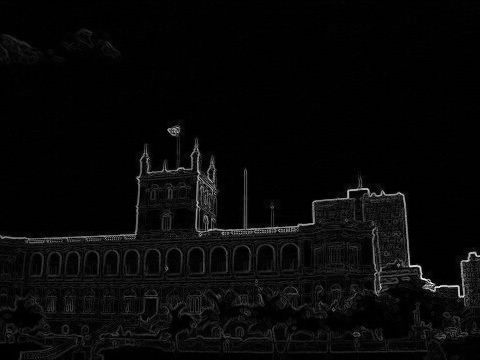
\includegraphics[width=150px]{./img/magnitude.jpg}	
		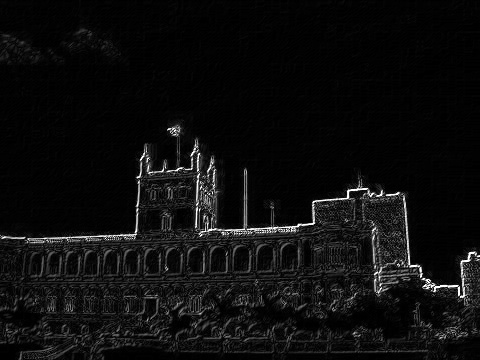
\includegraphics[width=150px]{./img/magnitude_3.jpg}	
		\caption{Porovnání magnitud. Vlevo magnituda z POEMU, vpravo magnituda z barevného POEMU.}
\end{figure}


\subsection{Diskretizace směru gradientu u barevneho poemu}
U vektorů získaných v předchozím kroku je určena velikost úhlu mezi vektorem a equivalentní vektorem s vynulovanou složkou $z$. Následně je spočítáno do které části kružnice vektor směřuje. Pro znaménkovou reprezentaci je celkový rozsah $0 - \pi$, pro neznaménkovou reprezentaci $0 - 2\pi$
\\
Při neznaménkové reprezentaci a počtu směrů $d = 3$, jsou následující intervaly $\left(0 - \frac{\pi}{3}\right)$, $\left(\frac{\pi}{3} - \frac{2\pi}{3}\right)$ a  $\left(\frac{2\pi}{3} - \pi\right)$.

\begin{figure}[H]
    \centering    
    \def\svgwidth{\columnwidth}
	\import{img/}{3D_kruznice.pdf_tex}    
    %\input{image.pdf_tex}
    \caption{Diskretizace směru gradientu v neznamenkové reprezentaci. Mějme vektor $[4, 9, 8]$ a jeho ekvivalentní vektor s vynulovanou složkou $z$ $[4,9, 0]$. Úhel, který mezi sebou vektory svírají je $39 ^\circ$. Zároveň je vektor v prvním kvadrantu tudíž spadá do prvního intervalu.}
    \label{fig: diskretizace3D}
\end{figure}

\par Pro výpočet diskretizace směru při neznaménkové reprezentaci je $y$ složka rozdělena na kladnou a zápornou část. To hraje velkou roli, pokud je $y$ složka vekotru záporná. V tom případě je nutné nebrat úhel $\alpha$, ale jeho doplněk ($ 180 - \alpha$).

\subsection{Výpočet lokálního histogramu u barevneho poemu}
Zbývající postup je již totožný s výše uvedeným POEM. Pro srovnání jsou zde alespoň uvedeny výsledné obrázky. 

\begin{figure}[H]
	\centering
	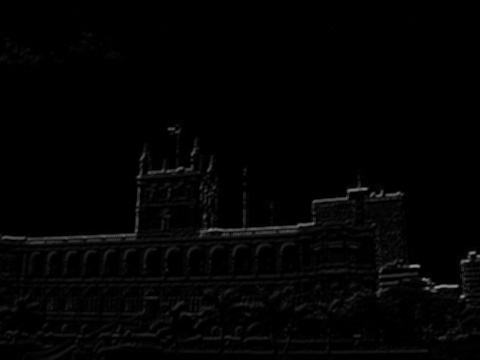
\includegraphics[width=150pt]{./img/aems0.jpg}
	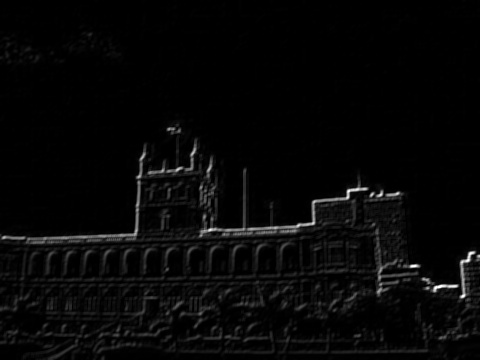
\includegraphics[width=150pt]{./img/aems_3_0.jpg}
	\caption{Obrázky po diskretizaci první směr. Vlevo původní POEM, vpravo barevný POEM}
\end{figure}
\begin{figure}[H]
	\centering
	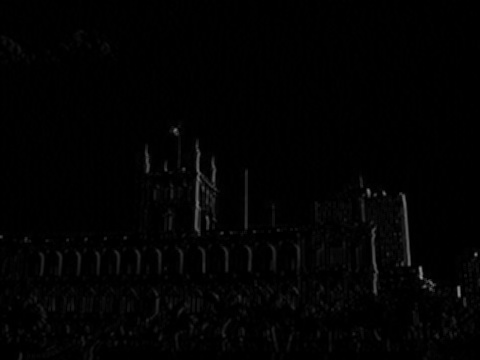
\includegraphics[width=150pt]{./img/aems1.jpg}
	
\includegraphics[width=150pt]{./img/aems_3_1.jpg}
	\caption{Obrázky po diskretizaci druhý směr. Vlevo původní POEM, vpravo barevný POEM}
\end{figure}
\begin{figure}[H]
	\centering	
	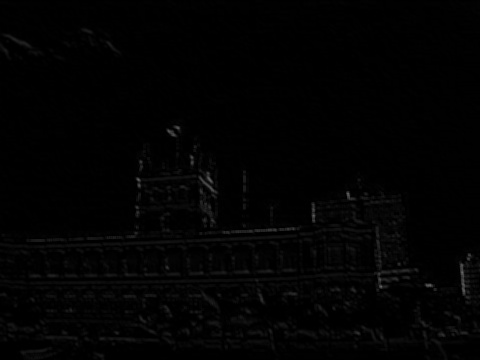
\includegraphics[width=150pt]{./img/aems2.jpg}
	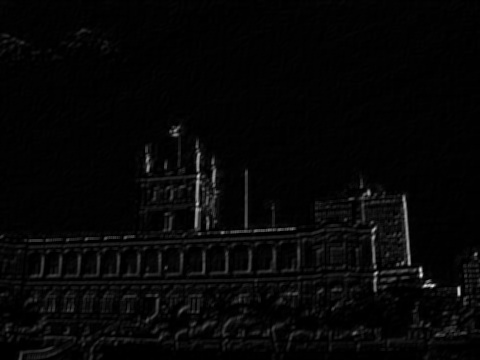
\includegraphics[width=150pt]{./img/aems_3_2.jpg}
	\caption{Obrázky po diskretizaci první směr. Vlevo původní POEM, vpravo barevný POEM}
\end{figure}

\subsection{Zakódování příznaku pomocí LBP u barevneho poemu}
\begin{figure}[H]
	\centering
	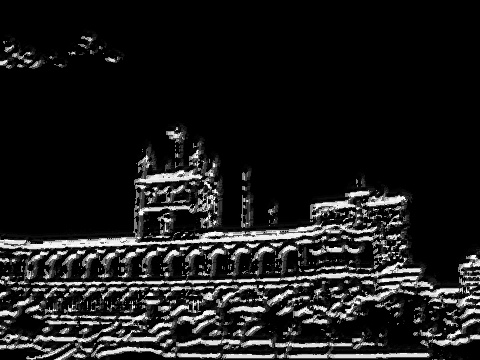
\includegraphics[width=150pt]{./img/lbp0_tau.jpg}
	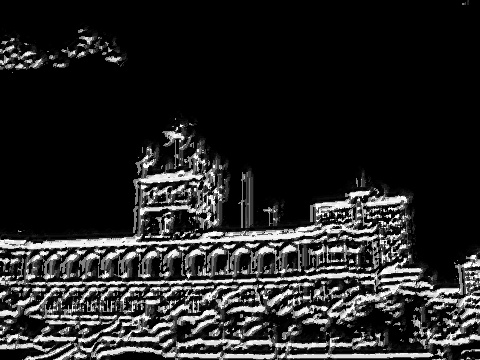
\includegraphics[width=150pt]{./img/lbp_3_0.jpg}
	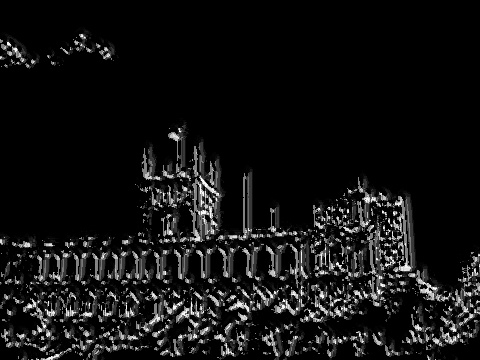
\includegraphics[width=150pt]{./img/lbp1_tau.jpg}
	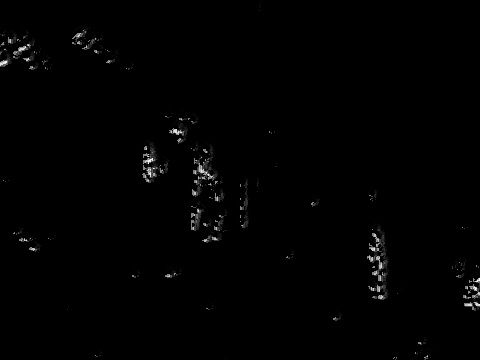
\includegraphics[width=150pt]{./img/lbp_3_1.jpg}
	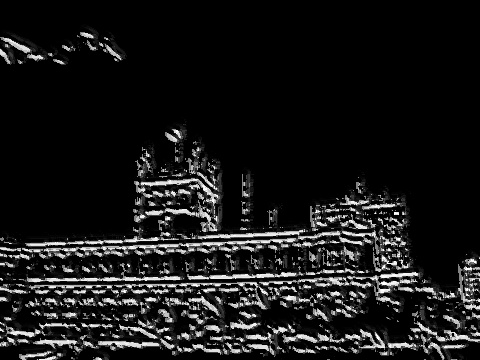
\includegraphics[width=150pt]{./img/lbp2_tau.jpg}
	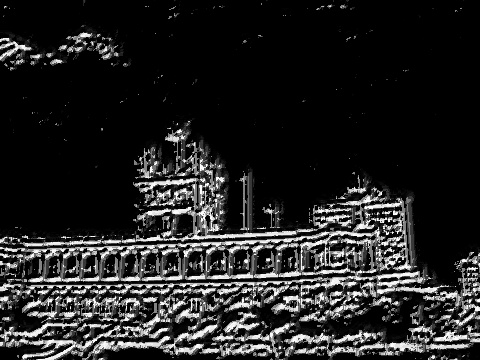
\includegraphics[width=150pt]{./img/lbp_3_2.jpg}
	\caption{Obrázky po aplikaci LBP s použitím $\tau$. Vlevo původní POEM, vpravo barevný POEM}
\end{figure}

\chapter{Použité programové prostředky}
Program byl navržen na operační systému Linux. Jako programovací jazyk byl zvolen Python a to z důvodu jeho jednoduchého použití, což je na prototyp, jako je tento velice výhodné na časovou náročnost. Počítač na kterým byl program vyvíjen a spouštěn pracoval s Python verzí 2.7.12. Program využívá knihovnu OpenCV 3.1. 
  
\section{OpenCV}
OpenCV (Open source computer vision) je knihovna vydávána pod licencí BSD a je volně k dispozici jak pro akademické účely, tak pro komerční použití. Je vhodná pro použití v C++, C, Python a Javě. Podporuje operační systémy Windows, Linux, Mac OS, iOS a Android.
\\
Knihovna byla navrhnuta pro výpočetní efektivitu v oblasti počítačového vidění a zpracování obrazu se zaměřením na zpracování obrazu v reálném čase. Z důvodu optimalizace byla napsána v C/C++. 
\\
Knihovnu OpenCV je možné stáhnout na adrese: \url{http://opencv.org/}  

\chapter{Testovací data}
Pro natrénování a následné testování byla použita data z databáze iaprc12. Data obsahují \num{20 000} obrázků ve formátu \textit{jpg} s celkovým počtem 291 klíčových slov. Z toho bylo použito \num{19 805} obrázků a to \num{17 664} na trénování a \num{1 960} na testování. K jednomu obrázku je v průměru přiřazeno 5.7 klíčových slov.\\

Ke každému obrázku jsou přiložena metadata ve formátu XML, která obsahují informace o obrázku v různých jazycích. Kromě angličtiny je zde možné nalést například i španělštinu nebo němčinu. Metadatata ovšem neobsahují klíčová slova, ale v jednotlivých elementech jsou roztřízené obsáhle informace. Například titulek obrázku, který může vypadat \textit{The Plaza de Armas}, a v elementu \textit{description} je například \textit{a woman and a child are walking over the square}. Spolu s databází byla získána i klíčová slova které byla extrahována právě z přiloženého xml.

\begin{figure}[h]
		\centering
		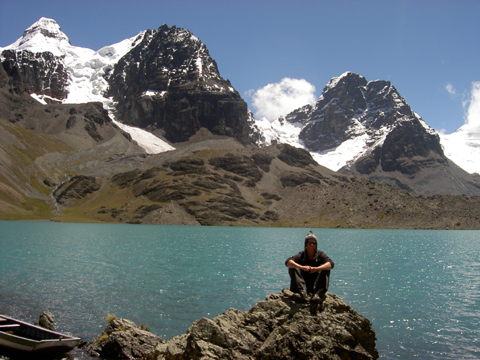
\includegraphics[width=140px]{./img/iaprtc12.jpg}	
		\caption{Ukázka obrázku s klíčovými slovy: front lake man mountain rock sky summit}
\end{figure}
 
\chapter{Závěr}
V semestrální práci byl vytvořen skript, který z vloženého obrázku vytvoří POEM deskriptor. Dále bylo vyzkoušeno vytvoření POEM na barevný obrázek, tak aby obsahoval jak informaci o textuře tak informaci o barvě. Použitý POEM byl použit pro porovnání v bakalářské práci \textit{Automatická anotace obrázků}. \\
\\
Dosažené výsledky: \\
Při spojování bylo použito Joint Equal Contribution. \cite{JEC} 

\begin{tabular}{l*{3}{c}}
	          		& Přesnost (\%) & Úplnost (\%) & Nenulových slov \\
\hline
RGB						& 14 & 8 & 167 \\
LAB	  			  		& 12 & 7 & 148  \\
HSV            			& 16 & 10 & 181  \\
RGB, LAB, HSV      		& 17 & 11 & 178  \\
POEM		     		& 0 & 0 & 0  \\
RGB, LAB, HSV, POEM		& 0 & 0 & 0  \\
Barevný POEM			& 0 & 0 & 0  \\
\end{tabular}


\chapter{Uživatelská dokumentace}
Pro spuštění programu je třeba mít nainstalovaný python (2.7.12) a knihovnu openCV verzi 3.1. Následné postupy jsou uvedeny pro operační systém Linux.

\subsubsection{Spuštění programu}
Program spustíme z příkazové řádky zadáním příkazu \textit{python nazevskriptu.py}. 
\begin{itemize}
	\item \textit{python poem.py obrazek.jpg} - v případě poemu pracujícím s šedotónovým obrázkem
	\item \textit{python color\_poem.py obrazek.jpg} - v případě poemu pracujícím s barevným obrázkem
\end{itemize}

\subsubsection{Výstupy programu}
V případě zájmu se můžeme podívat na mezivýstupy programu.
\begin{itemize}
	\item \textit{gradientX.jpg} - obrázek po použití filtru x, analogicky \textit{gradientY.jpg}
	\item \textit{gradientX.txt} - matice po použití filtru x, analogicky \textit{gradientY.txt} 
	\item \textit{magnitude.jpg} - obrázek vzniklý po spočtení magnitud
	\item \textit{magnitude.txt} - matice magnitud 
	\item \textit{phase.txt} - matice magnitud 
	\item \textit{directional1.jpg} - obrázek magnitud po rozdeleni do smeru, smer 1 (analogicky directional2.jpg, atd)
	\item \textit{directional1.txt} - magnitudy po rozdeleni do smeru, smer 1 (analogicky directional2.txt, atd)
	\item \textit{ames1.jpg} - obrázek po výpočtu lokálních histogramů orientace gradientů, smer 1 (analogicky aems2.jpg, atd)
	\item \textit{ames1.txt} - matice po výpočtu lokálních histogramů orientace gradientů, smer 1 (analogicky aems2.txt, atd)
	\item \textit{lbp1.jpg} - obrázek výsledného LBP, smer 1 (analogicky lbp2.jpg, atd)
	\item \textit{lbp1.txt} - výsledného LBP, smer 1 (analogicky lbp2.txt, atd)
\end{itemize}

\bibliography{literatura}

\end{document}